
%%% This project is made by BoWang (School of Automation, HDU)
%%%%%%%%%%%%%%%%%%%%%%%%%%%%%%%%%%%%
%%bachelor_p %%%%%%本科生模板
%%master_p %%%%%%硕士生模板
%%doctor_p %%%%%%博士生模板
%%course_p %%%%%%课程报告、课程实验报告、课程思政报告
%%%%%%%%%%%%%%%%%%%%%%%%%%%%%%%%%%%%%%%%%%%%%%%%%%%%%%%%%%%%%%%%%%%%%%%%%%%%%%%%%%%%%%%

\documentclass[bachelor_p]{open-report}

\title{杭州电子科技大学Latex毕业论文模板使用方法}{Munual of latex on thesis for HDU}%%%题目,英文部分{}内可以不填
\author{张三}{San Zhang}%%%%%%作者,英文部分{}内可以不填
\advisor{王老师}{Teacher Wang}%%%%%%指导老师,英文部分{}内可以不填
\school{自动化学院}{School of Automation}%%%%学院,英文部分{}内可以不填
\major{控制科学与工程}{Control Science and Engineering}%%%%%%%%%%专业,英文部分{}内可以不填
\authornumber{20212021}%%%%%%学号
\authorclass{171819} %%%%%%%%%班级
% \course{机器学习}{思政报告} %%%%非开题报告填写:第一项课程名称,第二项写报告类型,如实验报告、思政等
% \completedate{2022}{2}{Feb}  %%%%%%设计完成时间
%%%%%%%%%%%%%%%%%%%%%%%%%%%%%%%%%%%%%%%%%%%%%%%%%%%%%%%%%%%%%%%%%%%%%

\begin{document}
%%%%%%%%%%%加载封面%%%%%%%%%%%%%%%%%%%%%%%%%%
\makecover
%%%%%%%%%%%%%%%%%%%%%%%%%%%%%%%%%%%%%%%%%


% %%%%%%%%%%%%%%%%%%%%%%%%%%%%%%%%%%%%%%%%%标题%%%%%%%%%%%%%%%%%%%%%%%%%%%%%%%%%%%%
\reporttitle

%%%%%%%%%%%%%%%%%%%%%%%%%%%%%%%%%%%%%%%%%%%%%%%%%%%%%%%%%%%%%%%%%%%%%%%%%%%%%%%%%%%%%%%

% %%%%%%%%%%%%%%%%%%%%%%%%%%%%%%%%%%%%%%%%%%%%%%%%%%%%%%%%%%%%%%%%%%%%%%%%%%%%%%%%%%%%%
% %%%%%%%%%%%%%%%%%%%%%%%%%%%%%%%%%%%%%%%%正文%%%%%%%%%%%%%%%%%%%%%%%%%%%%%%%%%%%%
%%%%%%%%%%%%%%%%%%%%%%%%%%%%%%研究现状%%%%%%%%%%%%%%%%%%%%%%%%%%%%%%%%%%
\section{\introduction}
%%%%%%%%%%%%%%%%%%%%%%%%%%%%%%%%%%%%%%%%%%%%%%%%%%%%%%

\subsection{1. 研究背景和意义}

latex的具体使用方法,请参考本科毕业设计latex模板的详细说明。通过命令\verb+`\vspace{20cm}`+空20cm的距离适当调整段间距离,保证和word模板一致。


\subsubsection{1.1 参考文献引用说明}
参考文献有两种格式引入\verb+\cite{}+以及\verb+\citep{}+。使用效果可见下面介绍:\\
参考文献有两种格式引入\verb+\cite{}+以及\verb+\citep{}+。使用效果可见下面介绍:\\
1.插入会议inproceedings\cite{zhao2015bearing0}\\
2.插入教材课本book\cite{williams1991probability,chengzhaolin2006,zhangsan2007}\\
3.插入期刊article\cite{cao2011formation,xue2015formation}\\
4.插入硕博论文thesis\cite{lisi2015,wangwu2015,deans2005bearings}\\
5.插入网站misc\cite{irdawebsite,h7n9,wikipedia_moores_law}\\
6.插入专利patent\cite{xiao2012yi,p6915001}\\
7.插入新闻news报纸newspaper\cite{zhang2000,renminribao}\\
8.插入标准standard\cite{gbt3469-1983}
\textcolor{red}{注意:参考文献格式不正确可能导致编译不通过,大家可以参考本工程中reference.bib中文献格式对网上下载不规范的bibtex文件进行修改。此外,如果上述类型里面条目有缺失会会导致编译不能输出正确格式。}关于参考文献不同类型的进一步详细的说明可参考网站https://github.com/Haixing-Hu/GBT7714-2005-BibTeX-Style
里面的测试模板。



\textcolor{red}{注意1:参考文献格式不正确可能导致编译不通过,大家可以参考本工程中reference.bib中文献格式对网上下载不规范的bibtex文件进行修改。此外,如果上述类型里面条目有缺失会会导致编译不能输出正确格式。}

关于参考文献不同类型的进一步详细的说明可参考网站https://github.com/Haixing-Hu/GBT7714-2005-BibTeX-Style
里面的测试模板。


\textcolor{red}{注意2:对于中文参考文献,为了保证格式正确,最好需在对应bib里面添加language={zh},不加会默认当做英文文献处理。区别如图\ref{fig_bib0}。}

\begin{figure}[!htb]
  \centering
  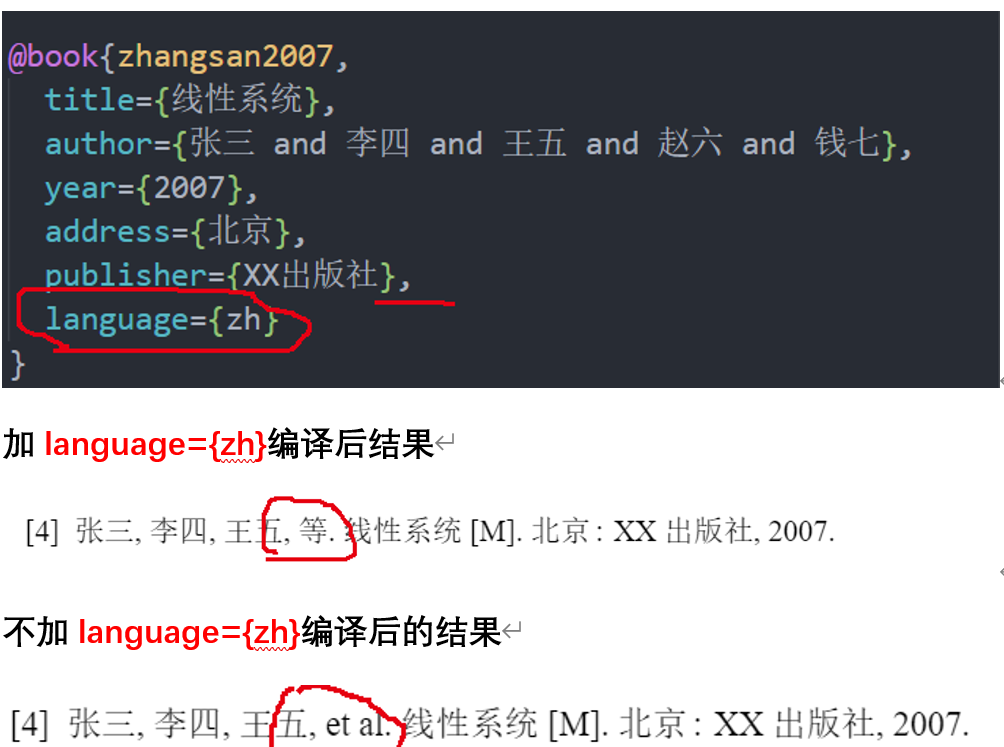
\includegraphics[width=1\textwidth]{中英文文献bib编译注意事项}
  \caption{中英文文献bib编译注意事项以作者超过3个为例进行说明}
  \label{fig_bib0}
\end{figure}


\subsubsection{1.2 参考文献的查找与引用}


多智能体系统\citep{cao2011formation}。
可以通过百度学术搜索查找参考文献(如图\ref{fig_search0}),
 \begin{figure}[!htb]
  \centering
  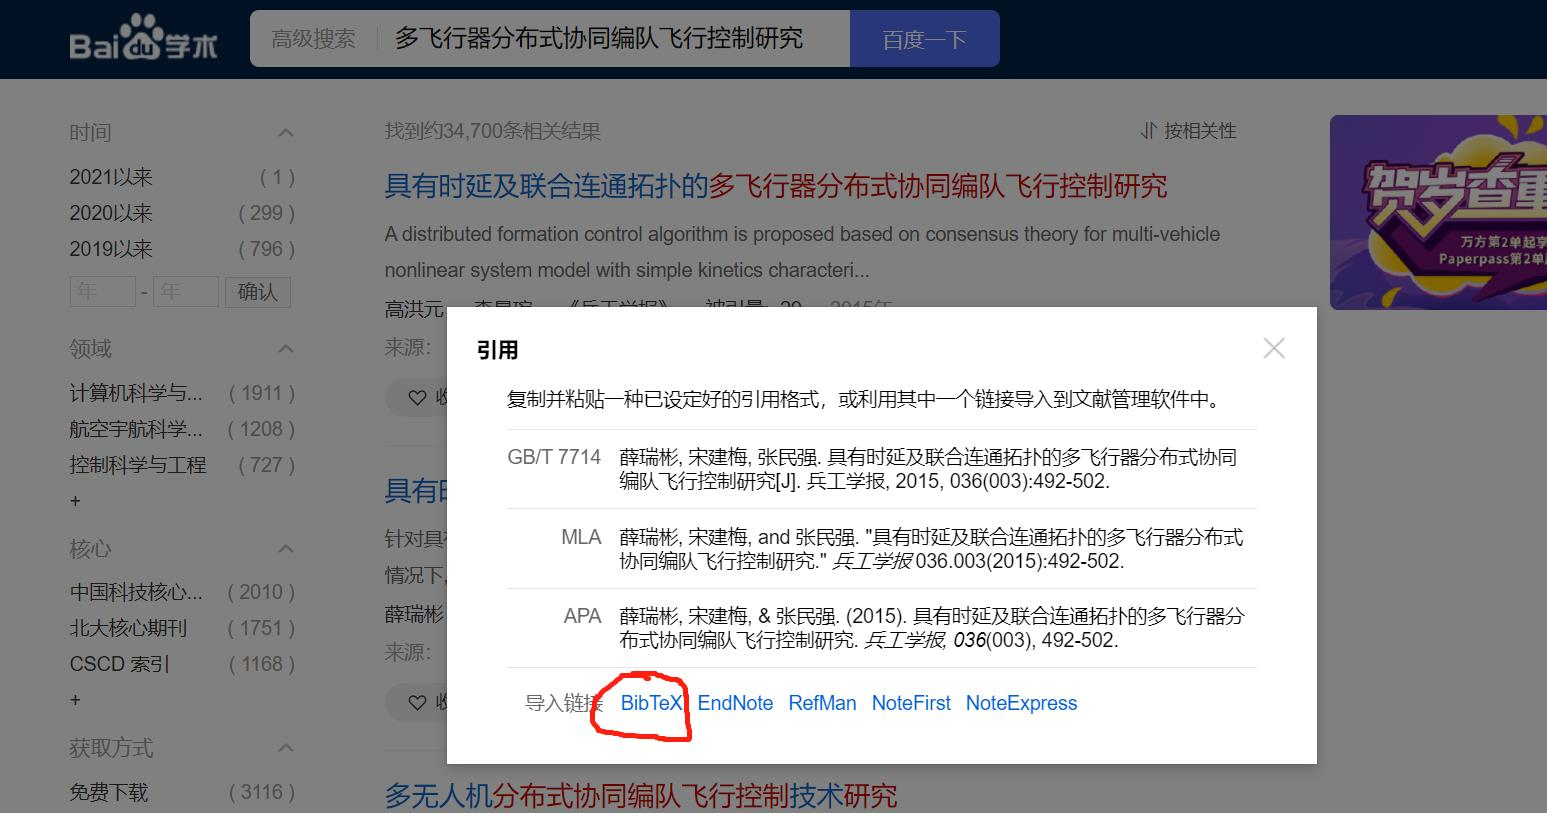
\includegraphics[width=1\textwidth]{文献搜索说明0}
  \caption{参考文献的百度学术搜索.}
  \label{fig_search0}
\end{figure}
点击bibtex,然后复制到目录文件夹中的bib文件(如图\ref{fig_search1})。此时可以调用指令为\citep{薛瑞彬2015具有时延及联合连通拓扑的多飞行器分布式协同编队飞行控制研究}。但是此时标签太长,可以适当修改标签再引用,例如把bib中的标签(第一行)的``薛瑞彬2015具有时延及联合连通拓扑的多飞行器分布式协同编队飞行控制研究"改成``xue2015formation",指令为\verb+\cite{xue2015formation}+,效果为\cite{xue2015formation}。如果进一步想管理参考文献,可新建几个bib文件并用\verb+\bibliography{en_ref,cn_ref,...}+完成。
 \begin{figure}[!htb]
  \centering
  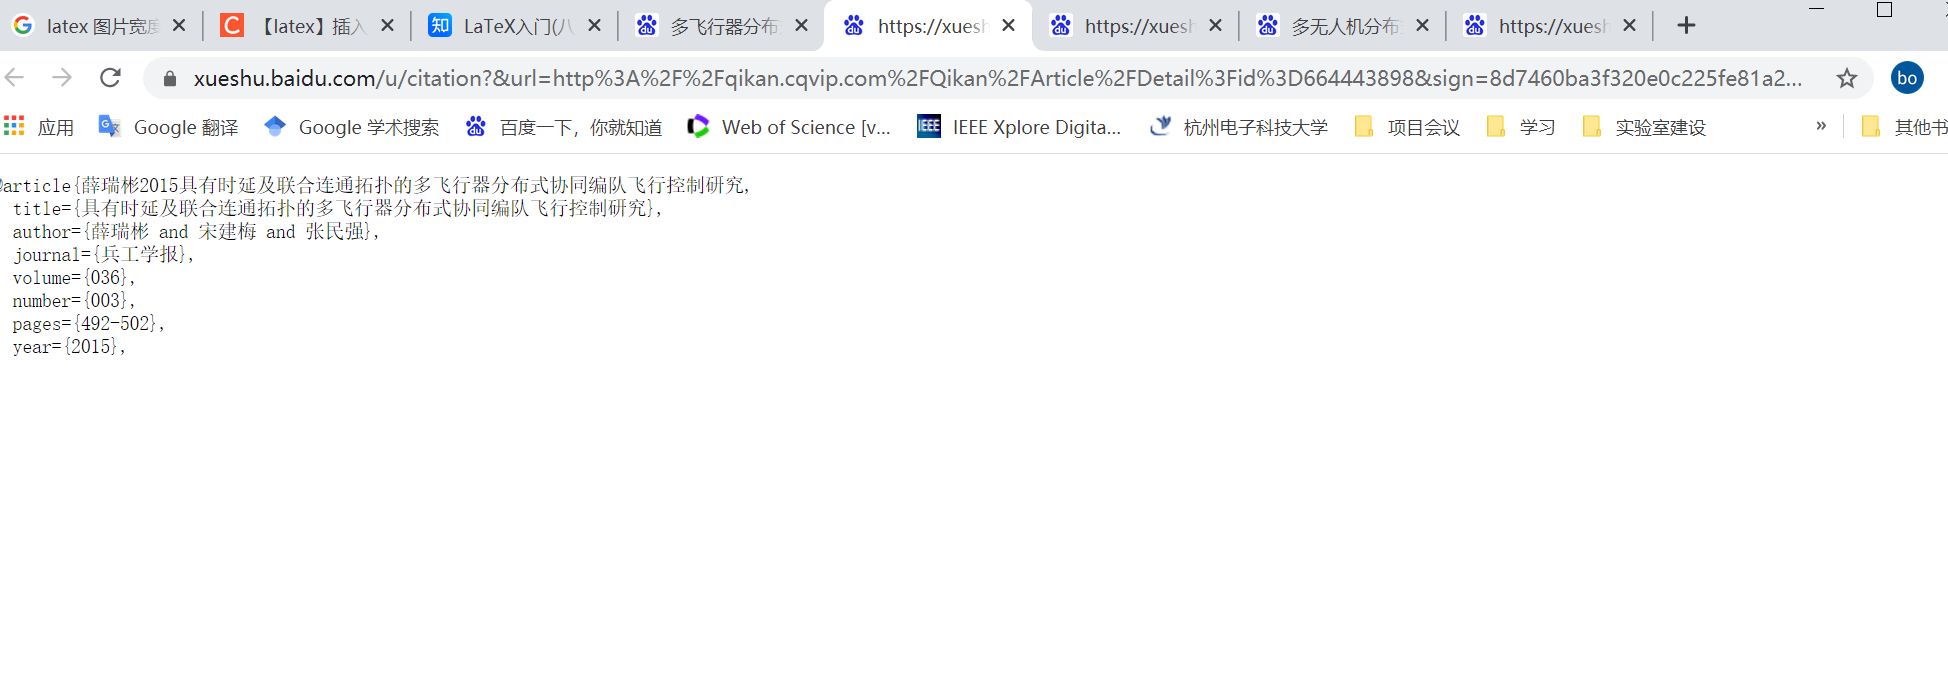
\includegraphics[width=1\textwidth]{文献搜索说明1}
  \caption{参考文献复制到bib文件.}
  \label{fig_search1}
\end{figure}









\subsection{2. 国内外研究现状}

得到的研究取得了重要进展。

%%%%%%%%%%%%%%%%%%%%%%%%%%%%%%研究内容%%%%%%%%%%%%%%%%%%%%%%%%%%%%%%%%%%%%%%
\section{\content}
%%%%%%%%%%%%%%%%%%%%%%%%%%%%%%%%%%%%%%%%%%%%%%%%%%%%%%%%%%%%%%%%%%%%%%%%%%%
将研究内容写在这里,可以直接输入,或通过文件引入如下所示:
% !Mode:: "TeX:UTF-8"

\section{研究的基本内容,拟解决的主要问题}


\subsection{插入项目符号}

多智能体系统在多方面多领域得到了广泛的应用:
\begin{itemize}
  \item 军事
  \item 政治
  \item 历史
\end{itemize}

\subsection{插入项目编号}

%% enumerate看效果\Alph*,\alph*,\Roman*,\roman*,\arabic*
多智能体系统的分类:
\begin{enumerate}[label=\alph*)]   
  \item 同构多智能体系统
  \item 异构多智能体系统
\end{enumerate}




\subsection{公式的对齐与引用}

\subsection{安装mathtype}
安装mathtype并根据下图完成配置(图\ref{fig_mathtype1}所示)。
 \begin{figure}[!htb]
  \centering
  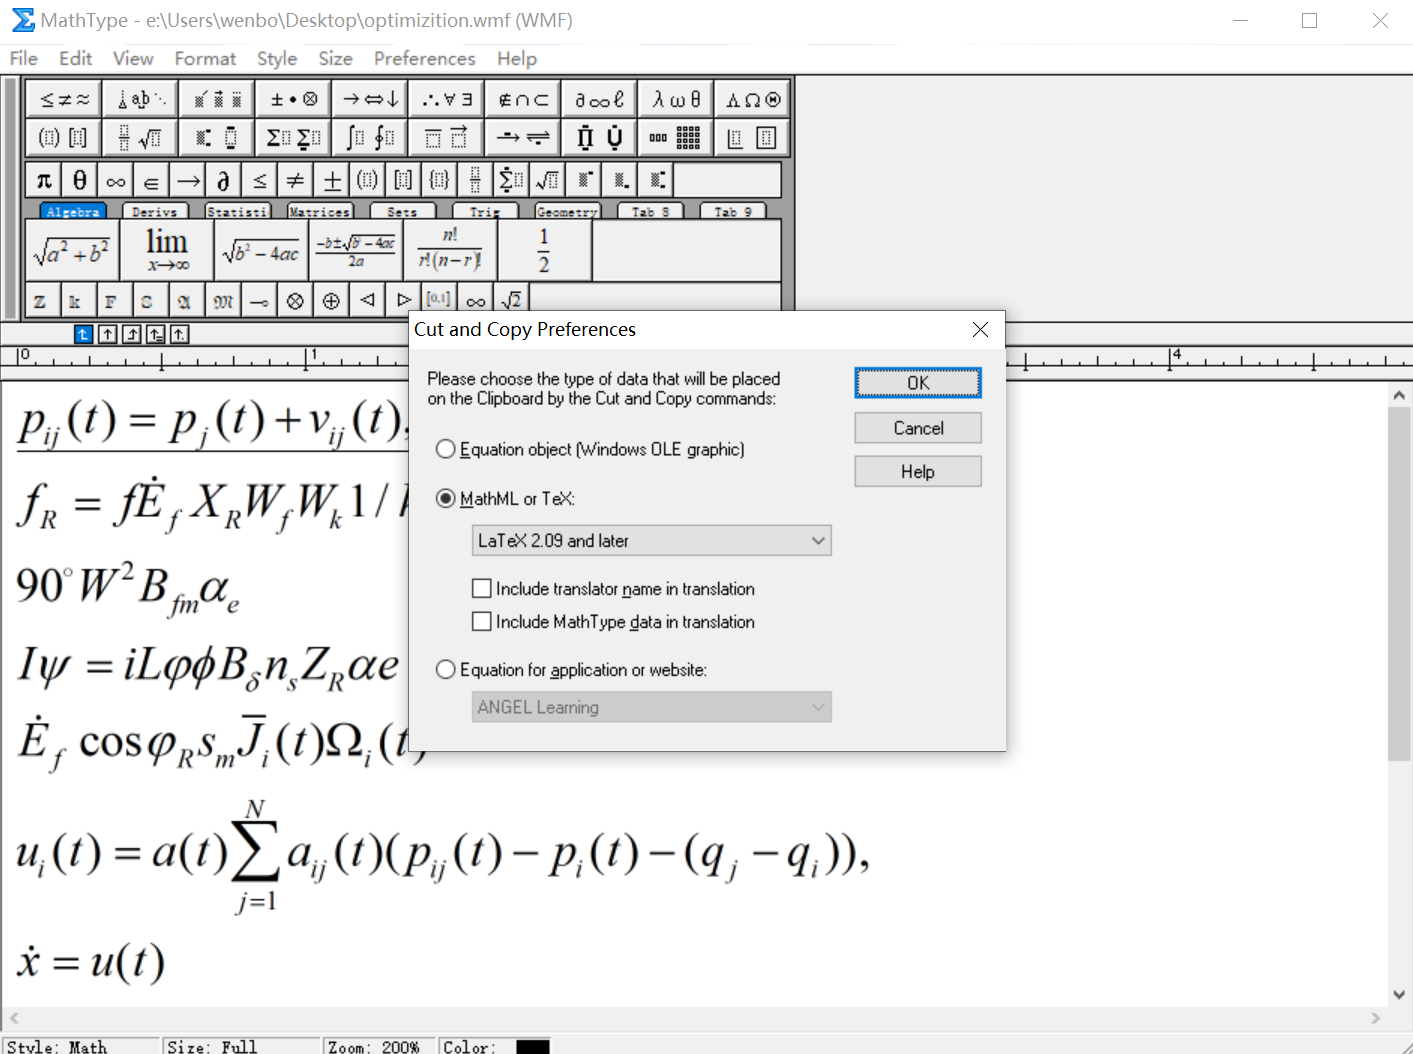
\includegraphics[width=1\textwidth]{mathtype配置}
  \caption{mathtype相关配置.}
  \label{fig_mathtype1}
\end{figure}

\subsection{插入带编号的公式及不带编号的公式}
在mathtype编辑公式,并从mathtype直接复制到latex,然后进一步修改。

\textcolor{red}{在文字段落中嵌入公式},此时需用到\$符号。下面是详细步骤,首先从mathtype中直接复制过来,不做任何修改,直接编译效果如下
\[{p_{ij}}(t) = {p_j}(t) + {v_{ij}}(t)\]
\textcolor{red}{如果嵌入到一段文字中},需要去掉 \verb|\[|以及\verb|\]|符号,然后用\$包起来,效果是${p_{ij}}(t) = {p_j}(t) + {v_{ij}}(t)$。

如果不嵌入在一段文字中,让公式单独成行,并编号,可以采用下列步骤。
下面公式是直接复制过来,未加任何修改的编译效果。
\[\begin{array}{l}
V(k) \ge \mathop {\min }\limits_{i \in {\cal V}} {\pi _i}(k)\sum\limits_{i = 1}^N {{{({x_i}(k) - {\pi ^T}(k)x(k))}^2}} \\
 \ge \frac{1}{2}\mathop {\min }\limits_{i \in {\cal V}} {\pi _i}(k){(\mathop {\max }\limits_{i \in {\cal V}} {x_i}(k) - \mathop {\min }\limits_{i \in {\cal V}} {x_i}(k))^2}\\
 \ge \frac{1}{2}\mathop {\min }\limits_{i \in {\cal V}} {\pi _i}(k)(\mathop {\max }\limits_{i \in {\cal V}} {x_i}(k)\\
 \ge \frac{1}{2}\mathop {\min }\limits_{i \in {\cal V}} {\pi _i}(k)(\mathop {\max }\limits_{i \in {\cal V}} {x_i}(k)
\end{array}\]



首先需要去掉 \verb|\[|以及\verb|\]|符号,然后用\verb+\begin{equation}以及\end{equation}+来替换。
\begin{equation}\label{system1}
  \begin{array}{l}
V(k) \ge \mathop {\min }\limits_{i \in {\cal V}} {\pi _i}(k)\sum\limits_{i = 1}^N {{{({x_i}(k) - {\pi ^T}(k)x(k))}^2}} \\
 \ge \frac{1}{2}\mathop {\min }\limits_{i \in {\cal V}} {\pi _i}(k){(\mathop {\max }\limits_{i \in {\cal V}} {x_i}(k) - \mathop {\min }\limits_{i \in {\cal V}} {x_i}(k))^2}\\
 \ge \frac{1}{2}\mathop {\min }\limits_{i \in {\cal V}} {\pi _i}(k)(\mathop {\max }\limits_{i \in {\cal V}} {x_i}(k)\\
 \ge \frac{1}{2}\mathop {\min }\limits_{i \in {\cal V}} {\pi _i}(k)(\mathop {\max }\limits_{i \in {\cal V}} {x_i}(k)
\end{array}
\end{equation}

\textcolor{red}{插入不带编号的公式},只需将equation改成\verb+equation*+
\begin{equation*}
  \begin{array}{l}
V(k) \ge \mathop {\min }\limits_{i \in {\cal V}} {\pi _i}(k)\sum\limits_{i = 1}^N {{{({x_i}(k) - {\pi ^T}(k)x(k))}^2}} \\
 \ge \frac{1}{2}\mathop {\min }\limits_{i \in {\cal V}} {\pi _i}(k){(\mathop {\max }\limits_{i \in {\cal V}} {x_i}(k) - \mathop {\min }\limits_{i \in {\cal V}} {x_i}(k))^2}\\
 \ge \frac{1}{2}\mathop {\min }\limits_{i \in {\cal V}} {\pi _i}(k)(\mathop {\max }\limits_{i \in {\cal V}} {x_i}(k)\\
 \ge \frac{1}{2}\mathop {\min }\limits_{i \in {\cal V}} {\pi _i}(k)(\mathop {\max }\limits_{i \in {\cal V}} {x_i}(k)
\end{array}
\end{equation*}


\subsection{公式对齐}

但是发现以上的公式并不美观,可以进一步进行对齐完善,\textcolor{red}{仔细对比\eqref{system1}公式代码和\eqref{system2}公式代码的区别},主要先删掉\verb+\begin{array}{l}+以及\verb+\end{array}{l}+,然后要在对齐的地方插入$\&$符号并结合\verb+\begin{split}+指令,完成对齐。

\begin{equation}\label{system2}
\begin{split}
V(k) &\ge \mathop {\min }\limits_{i \in {\cal V}} {\pi _i}(k)\sum\limits_{i = 1}^N {{{({x_i}(k) - {\pi ^T}(k)x(k))}^2}} \\
 &\ge \frac{1}{2}\mathop {\min }\limits_{i \in {\cal V}} {\pi _i}(k){(\mathop {\max }\limits_{i \in {\cal V}} {x_i}(k) - \mathop {\min }\limits_{i \in {\cal V}} {x_i}(k))^2}\\
 &\ge \frac{1}{2}\mathop {\min }\limits_{i \in {\cal V}} {\pi _i}(k)(\mathop {\max }\limits_{i \in {\cal V}} {x_i}(k)\\
 &\ge \frac{1}{2}\mathop {\min }\limits_{i \in {\cal V}} {\pi _i}(k)(\mathop {\max }\limits_{i \in {\cal V}} {x_i}(k).
\end{split}
\end{equation}

\textcolor{red}{公式太长的情形,一行放不下的公式,可参考以下进行修改(参考源latex代码进行区分二者的区别)。}举例1如下,下面第一个式子是直接从mathtype复制,第二个式子插入了标签同时进行了对齐(关键看式中的\&符号插入位置和符号$\backslash$$\backslash$的关系)\verb+\hspace{0.3cm}+来表示对齐时空0.3cm


\[\begin{array}{l}
V(k) \ge \mathop {\min }\limits_{i \in {\cal V}} {\pi _i}(k)\sum\limits_{i = 1}^N {{{({x_i}(k) - {\pi ^T}(k)x(k))}^2}} {\rm{ + }}\frac{1}{2}\mathop {\min }\limits_{i \in {\cal V}} {\pi _i}(k){(\mathop {\max }\limits_{i \in {\cal V}} {x_i}(k) - \mathop {\min }\limits_{i \in {\cal V}} {x_i}(k))^2}\\
{\rm{ + }}\frac{1}{2}\mathop {\min }\limits_{i \in {\cal V}} {\pi _i}(k){(\mathop {\max }\limits_{i \in {\cal V}} {x_i}(k) - \mathop {\min }\limits_{i \in {\cal V}} {x_i}(k))^2}
\end{array}\]

\begin{equation}\label{system3}
  \begin{split}
V(k) \ge& \mathop {\min }\limits_{i \in {\cal V}} {\pi _i}(k)\sum\limits_{i = 1}^N {{{({x_i}(k) - {\pi ^T}(k)x(k))}^2}} {\rm{ + }}\frac{1}{2}\mathop {\min }\limits_{i \in {\cal V}} {\pi _i}(k){(\mathop {\max }\limits_{i \in {\cal V}} {x_i}(k) - \mathop {\min }\limits_{i \in {\cal V}} {x_i}(k))^2}\\
&\hspace{0.3cm}{\rm{ + }}\frac{1}{2}\mathop {\min }\limits_{i \in {\cal V}} {\pi _i}(k){(\mathop {\max }\limits_{i \in {\cal V}} {x_i}(k) - \mathop {\min }\limits_{i \in {\cal V}} {x_i}(k))^2}
  \end{split}
\end{equation}

举例2如下
\[\begin{array}{l}
V(k) \ge \mathop {\min }\limits_{i \in {\cal V}} {\pi _i}(k)\sum\limits_{i = 1}^N {{{({x_i}(k) - {\pi ^T}(k)x(k))}^2}} {\rm{ + }}\frac{1}{2}\mathop {\min }\limits_{i \in {\cal V}} {\pi _i}(k){(\mathop {\max }\limits_{i \in {\cal V}} {x_i}(k) - \mathop {\min }\limits_{i \in {\cal V}} {x_i}(k))^2}\\
{\rm{ + }}\frac{1}{2}\mathop {\min }\limits_{i \in {\cal V}} {\pi _i}(k){(\mathop {\max }\limits_{i \in {\cal V}} {x_i}(k) - \mathop {\min }\limits_{i \in {\cal V}} {x_i}(k))^2}\\
 \ge \frac{1}{2}\mathop {\min }\limits_{i \in {\cal V}} {\pi _i}(k){(\mathop {\max }\limits_{i \in {\cal V}} {x_i}(k) - \mathop {\min }\limits_{i \in {\cal V}} {x_i}(k))^2}\\
 \ge \frac{1}{2}\mathop {\min }\limits_{i \in {\cal V}} {\pi _i}(k)(\mathop {\max }\limits_{i \in {\cal V}} {x_i}(k)
\end{array}\]




\begin{equation}\label{system4}
  \begin{split}
V(k) &\ge \mathop {\min }\limits_{i \in {\cal V}} {\pi _i}(k)\sum\limits_{i = 1}^N {{{({x_i}(k) - {\pi ^T}(k)x(k))}^2}} {\rm{ + }}\frac{1}{2}\mathop {\min }\limits_{i \in {\cal V}} {\pi _i}(k){(\mathop {\max }\limits_{i \in {\cal V}} {x_i}(k) - \mathop {\min }\limits_{i \in {\cal V}} {x_i}(k))^2}\\
&\hspace{2cm}{\rm{ + }}\frac{1}{2}\mathop {\min }\limits_{i \in {\cal V}} {\pi _i}(k){(\mathop {\max }\limits_{i \in {\cal V}} {x_i}(k) - \mathop {\min }\limits_{i \in {\cal V}} {x_i}(k))^2}\\
& \ge \frac{1}{2}\mathop {\min }\limits_{i \in {\cal V}} {\pi _i}(k){(\mathop {\max }\limits_{i \in {\cal V}} {x_i}(k) - \mathop {\min }\limits_{i \in {\cal V}} {x_i}(k))^2}\\
 &\ge \frac{1}{2}\mathop {\min }\limits_{i \in {\cal V}} {\pi _i}(k)(\mathop {\max }\limits_{i \in {\cal V}} {x_i}(k)
  \end{split}
\end{equation}


\subsection{定理环境}

定理插入可参考如下
\begin{theorem}
设$f$在凸集$D \subset {R^n}$上一阶连续可微,则
\begin{itemize}
\item $f$在$D$上为凸函数的充要条件是
\begin{equation*}
f(x) \ge f({x^*}) + \nabla f{({x^*})^T}(x - {x^*}),\forall {x^*},x \in D.
\end{equation*}
\item  $f$在$D$上严格凸的充要条件是$x \ne y$时,
\begin{equation*}
f(x) > f({x^*}) + \nabla f{({x^*})^T}(x - {x^*}),\forall {x^*},x \in D.
\end{equation*}
\item $f$在$D$上一致凸的充要条件是,存在常数$c > 0$,使得
成立
\begin{equation*}
f(x) > f({x^*}) + \nabla f{({x^*})^T}(x - {x^*}) + c{\left\| {x - {x^*}} \right\|^2},\forall {x^*},x \in D.
\end{equation*}
\end{itemize}
\end{theorem}

\subsection{定义环境}
\begin{definition}
设集合 $D \subset {R^n}.$ 称集合$D$为凸集, 是指对任意的 $x,y \in {R^n}$及任意
的实数$\lambda  \in [0,1],$ 都有$\lambda x + (1 - \lambda )y \in D.$
\end{definition}

\subsection{假设环境}
\begin{assumption}
设$f$在凸集$D \subset {R^n}$上一阶连续可微。
\end{assumption}
\subsection{问题环境}
\begin{problem}
  设$f$在凸集$D \subset {R^n}$上一阶连续可微。
  \end{problem}
 
\subsection{其它环境}
其它环境可参考下图配置
\textcolor{red}{插入引理、推论等可参考下图对定理环境做对应修改得到(如图\ref{fig_定理环境}所示}。
 \begin{figure}[!htb]
  \centering
  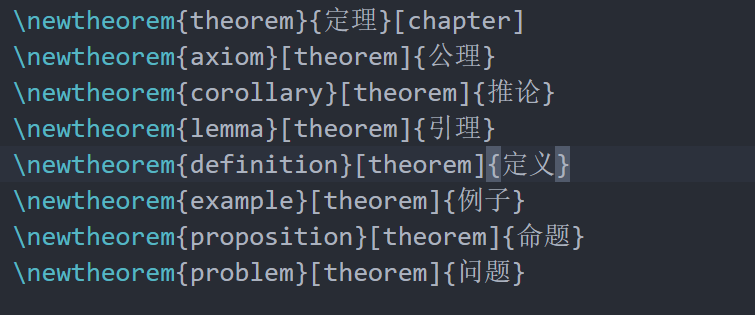
\includegraphics[width=1\textwidth]{定理环境}
  \caption{根据此图做对应修改可插入引理、推论等,具体代码可看latex开头部分环境定义}
  \label{fig_定理环境}
\end{figure}



\subsection{算法设计}

\begin{algorithm}[H]
    \KwIn {西瓜集}
    \KwOut{分类结果}
    初始化\;
    \While{迭代未终止}{
        学习\;
        \eIf{西瓜属性}{
            统计\;
            计算\;
        }{
            下一次迭代\;
        }
    }
    \caption{西瓜集分类算法}
\end{algorithm}



%%%%%%%%%%%%%%%%%%%%%%%%%%%研究方法%%%%%%%%%%%%%%%%%%%%%%%%%%%%%%%%%%%%%%%%
\section{\method}
%%%%%%%%%%%%%%%%%%%%%%%%%%%%%%%%%%%%%%%%%%%%%%%%%%%%%%%%%%%%%%%%%%%%%%%%%%%
将研究方法写这里
%%%%%%%%%%%%%%%%%%%通过插入下面命令来调整布局%%%%%%%%%%
\vspace{20cm}%%%%空20cm的距离
%%%%%%%%%参考文献%%%%%%%%%%%%%
%%%%%%%%%%%%%%%%研究进度%%%%%%%%
\section{\plan}

\begin{table}[h]
  \renewcommand\arraystretch{2}
  \centering
  \setlength{\tabcolsep}{12mm}{
  \begin{tabular}{|c|c|c|}
  \hline
  序号 & 时间                  & 内容      \\ \hline
  1  & 20xx.xx.xx-20xx.xx.xx & 任务书 \\ \hline
  2  & 20xx.xx.xx-20xx.xx.xx  & 撰写开题报告 \\ \hline
  3  & 20xx.xx.xx-20xx.xx.xx  & 开题报告会 \\ \hline
  4  & 20xx.xx.xx-20xx.xx.xx & 中期检查 \\ \hline
  5  & 20xx.xx.xx-20xx.xx.xx  & 撰写毕业论文 \\ \hline
  6  & 20xx.xx.xx-20xx.xx.xx  & 论文评审及查重 \\ \hline
  7  & 20xx.xx.xx-20xx.xx.xx   & 答辩报告会 \\ \hline
  8  & 20xx.xx.xx-20xx.xx.xx & 资料归档整理 \\ \hline
  \end{tabular}}
  \end{table}

%%%%%%%%%%%%%%%%%%%%%%%%%%%%%%%%%%%

%%%%%%%%%%%%%%%%%%%%%%%%%%%%%%%%%%%%%参考文献%%%%%%%%%%%%%
\reference
\vspace{-1cm}
\hdubibliography{ref/reference}

%%%%%%%%%%%%%%%%%%%%%%%%%%%%%%%%%%%%%%%%%%%%%%%%%%%%%%%%%%%%%%%%%%%%%
%%%%%%%%%%%%%%%%%%%%%%%%%%%%工作小组意见%%%%%%%%%%%%%%%%%%%%%%%%%%%%%%%%%%%
\newpage
\section{\comment}
%%%%%%%%%%%%%%%%%%%%%%%%%%%%%%%%%%%%%%%%%%%%%%%%%%%%%%%%%%%%%%%%%%%%%%%%%

\begin{table}[h]
  \large
  \renewcommand\arraystretch{1.5}
\begin{tabular}{|c|c|c|c|c|c|c|}
\hline
\textbf{\begin{tabular}[c]{@{}c@{}}考核\\点\end{tabular}} &
  \textbf{\begin{tabular}[c]{@{}c@{}}背景及意义\\ 阐述情况\end{tabular}} &
  \textbf{\begin{tabular}[c]{@{}c@{}}研究方案与任务\\ 书的匹配程度\end{tabular}} &
  \textbf{\begin{tabular}[c]{@{}c@{}}研究方法\\ 合理性\end{tabular}} &
  \textbf{\begin{tabular}[c]{@{}c@{}}进度安排\\ 情况\end{tabular}} &
  \textbf{\begin{tabular}[c]{@{}c@{}}答辩\\情况\end{tabular}} &
  \textbf{总分} \\ \hline
\textbf{\begin{tabular}[c]{@{}c@{}}对应\\课程\\ 目标\end{tabular}} &
  \textbf{\begin{tabular}[c]{@{}c@{}}课程\\目标1\end{tabular}} &
  \textbf{\begin{tabular}[c]{@{}c@{}}课程\\目标2\end{tabular}} &
  \textbf{\begin{tabular}[c]{@{}c@{}}课程\\目标3\end{tabular}} &
  \textbf{\begin{tabular}[c]{@{}c@{}}课程\\目标7\end{tabular}} &
  \textbf{\begin{tabular}[c]{@{}c@{}}课程\\目标5\end{tabular}} &
  \textbf{} \\ \hline
  \rule{0pt}{6ex}\textbf{满分} & \textbf{20} & \textbf{25} & \textbf{20} & \textbf{10} & \textbf{25} & \textbf{100} \\\hline
  \rule{0pt}{6ex}\textbf{评分} & \textbf{}   & \textbf{}   & \textbf{}   & \textbf{}   & \textbf{}   & \textbf{}    \\ \hline
\end{tabular}
\end{table}

\vspace{3cm}


\begin{flushright}

开题小组负责人签字:\_\_\_\_\_\_\_\_\_\_\_\_\ \ \ \

\vspace{1cm}
年\ \ \ \ \ \ 月\ \ \ \ \ \ 日\ \ \ \ \ \ \ \
\end{flushright}



\end{document}


